\chapter{Konzepte \& Architektur}
\label{ch:konzepte_architektur}
\section{Konzepte}
Für die Bewältigung der Anforderungen an die Softwarelösung wurden Konzepte entwickelt, welche Einfluss auf die einzelnen Komponenten und die Architektur haben. Die Softwarelösung soll wie unter \ref{ch:anforderungen_section} \nameref{ch:anforderungen_section} beschrieben,  die Möglichkeit bieten, Simulationsdaten auf einer Karte darzustellen, sowie auch deren Bearbeitung ermöglichen. Wichtig ist dabei, dass die Bearbeitung keinen Einfluss auf die Stammdaten hat. Die dafür benötigten Konzepte, werden in diesem Kapitel beschrieben.
\subsection{Daten QuadTiles}
\label{ch:datentiles}
Der Umgang mit der grossen Datenmenge (ca. 4 Millionen Datensätze für die Schweiz) ist eine grosse Herausforderung dieser Arbeit. Um diese grosse Datenmenge zu bewältigen, wurde ein bewährtes Verfahren für die Kartendarstellung verwendet. Dies ist der QuadTile Algorithmus von OpenStreetMap \citep{OSMQuadTiles}. Dabei werden die Daten nicht als Gesamtes geliefert, sondern über Teilbereiche, sogenannte Tiles, angefragt. Ein Tile ist ein Quadrat, welches ein vordefinierten Bereich der Welt abdeckt. Dies ermöglicht es einzelne Bereiche (Tiles), die zur Zeit angezeigt werden, zu laden und nicht immer den kompletten Datenstamm. Ein weiteres Konzept, in Verbindung mit dem QuadTile Algorithmus, wird unter \ref{sec:concept_preprocessing} \nameref{sec:concept_preprocessing} beschrieben. Dabei werden die Daten für jede Zoomstufe bewertet und lediglich bei Relevanz mitgeliefert. Durch diese beiden Konzepte kann die Datenmenge, die von der Website verarbeitet werden muss, stark reduziert werden.
\begin{figure}[H]
\centering
\includegraphics[height=7cm]{images/BingMapsTileSystem.jpg}
\\Quelle: \href{https://msdn.microsoft.com/en-us/library/bb259689.aspx}{https://msdn.microsoft.com/en-us/library/bb259689.aspx}
\caption{Fixe Aufteilung der Welt in Bereiche (Tiles)}
\label{fig:tilesystem}
\end{figure}
\noindent
Um von einem Datensatz (Link oder Node) auf das Tile zu schliessen, in welchem dieser sichtbar ist, wird ein Schlüssel (QuadKey) berechnet. Der QuadKey benennt eindeutig das kleinstmögliche Tile in welchem der komplette Datensatz ersichtlich ist. Der QuadKey setzt sich, wie in Abbildung \ref{fig:tilesystem} ersichtlich, aus der Nummerierung der Teilbereiche zusammen. Dabei wird die Welt in der äussersten Zoomstufe in 4 Bereiche aufgeteilt, die von 0 bis 3 durch nummeriert werden. Für die nächste Stufe, wird jeder Bereich aus Level 1 je wieder in 4 Bereiche aufgeteilt. Diese neuen Teilbereiche werden dann wieder nummeriert. Dabei wird die Nummerierung des vorhergehenden Bereichs als Prefix verwendet und wieder von 0 bis 3 durch nummeriert. Dadurch kann jeder Bereich auf jeder Zommstufe eindeutig adressiert werden. Dieser Algorithmus bietet ebenfalls die Möglichkeit, mit Hilfe des QuadKeys alle darunterliegenden Bereiche zu finden, weil dieser QuadKey ein Prefix aller QuadKeys ist, die unter diesem Bereich liegen. Dieser Ansatz wird für die Filterung der Daten verwendet.
\subsection{Preprocessing und Bewertung der Daten}\label{sec:concept_preprocessing}
Ein wichtiges Ziel der Aufbereitung der Daten, ist das verringern der Zugriffszeiten auf die Datenbank. Diese Aufbereitung findet direkt beim Import statt. Durch diesen Vorgang werden bewusst Redundanzen in das Datenmodell eingeführt. Diese Redundanzen erlauben den Zugriff auf Daten ohne teure JOIN Statements oder SQL-Funktionen aufzurufen. Auf die Berechnungen und Aufbereitungen, die beim Import des Datenmodells angewendet werden, wird genauer im Kapitel \ref{sec:tilingdataimplementation} \nameref{sec:tilingdataimplementation} eingegangen.
\newpage
\subsection{Changeset}\label{sec:changeset}
Der Benutzer kann auf dem Verkehrsmodell-Fallstudien-Editor Änderungen vornehmen und anschliessend persistieren. Dafür wurde ein Konzept entwickelt, dass es erlaubt Änderungen an den Daten abzuspeichern, ohne die Stammdaten direkt anzupassen. Arbeitet der Benutzer direkt mit den Stammdaten, hat dies zur Folge, dass für jeden Benutzer die gesamten Stammdaten separat abgelegt werden muss. Dies ist eine unnötige Redundanz der Daten und kostet unnötig viel Speicherplatz.\\
Um dem entgegen zu wirken, wird das Konzept Changeset verwendet. Dabei werden die Stammdaten nur einmalig abgelegt und von jedem Benutzer verwendet. Die Struktur eines Changesets stellt ein Abbild der Struktur der Stammdaten dar. Führt ein Benutzer eine Änderung an den Daten durch, wird lediglich die Differenz zu den Stammdaten in diesem Changeset abgelegt. Somit ist es möglich, wie in Abbilung \ref{fig:changeset_example} ersichtlich, das Changeset eines Benutzers als Differenz über die Stammdaten zu legen und somit den aktuellen Datensatz zu erhalten. Sollten Änderungen an den Stammdaten gemacht werden, sind diese direkt bei allen Benutzern ersichtlich, insofern die Änderungen nicht durch das Changeset überdeckt werden.
\begin{figure}[H]
\centering
\includegraphics[height=6cm]{images/Changeset.png}
\caption{Changeset Beispiel}
\label{fig:changeset_example}
\end{figure}
\noindent
\subsection{User Interface - Konzept}\label{sec:uiconcept}
Das User Interface ist eine zentrale Komponente des Verkehrsmodell-Fallstudien-Editors. Eine Voraussetzung für ein optimales User Interface, ist ein einfaches und intuitives Konzept, das ohne grosse Einarbeitungszeit zu bedienen ist. Für dieses Konzept diente Google Maps \cite{GoogleMaps} sowie auch der ID Editor \citep{IDEditor} von OpenStreetMap als Inspirationsquelle für das User Handling. Google Maps ist die am weitesten verbreitete Web Anwendung, wenn es um die Benutzung einer Karte im Browser geht. Für die Bearbeitung der Daten dient der oft genutzte ID Editor als Vorlage. Beide Web Applikationen besitzen ein durchdachtes Design, an dessen Bedienung sich die Benutzer gewöhnt sind.
\newpage
\subsubsection{Google Maps}
Google Maps ist eines der am weitesten verbreiteten Kartensystemen. Der Benutzer ist sich an das Handling von Google Maps gewöhnt und kann mit Systemen, die ähnlich aufgebaut sind, ohne Probleme arbeiten. Der grösste Vorteil von Google Maps ist die intuitive Bedienung, gekoppelt an ein einfaches, aufgeräumtes und leichtes Design.
\begin{figure}[H]
\centering
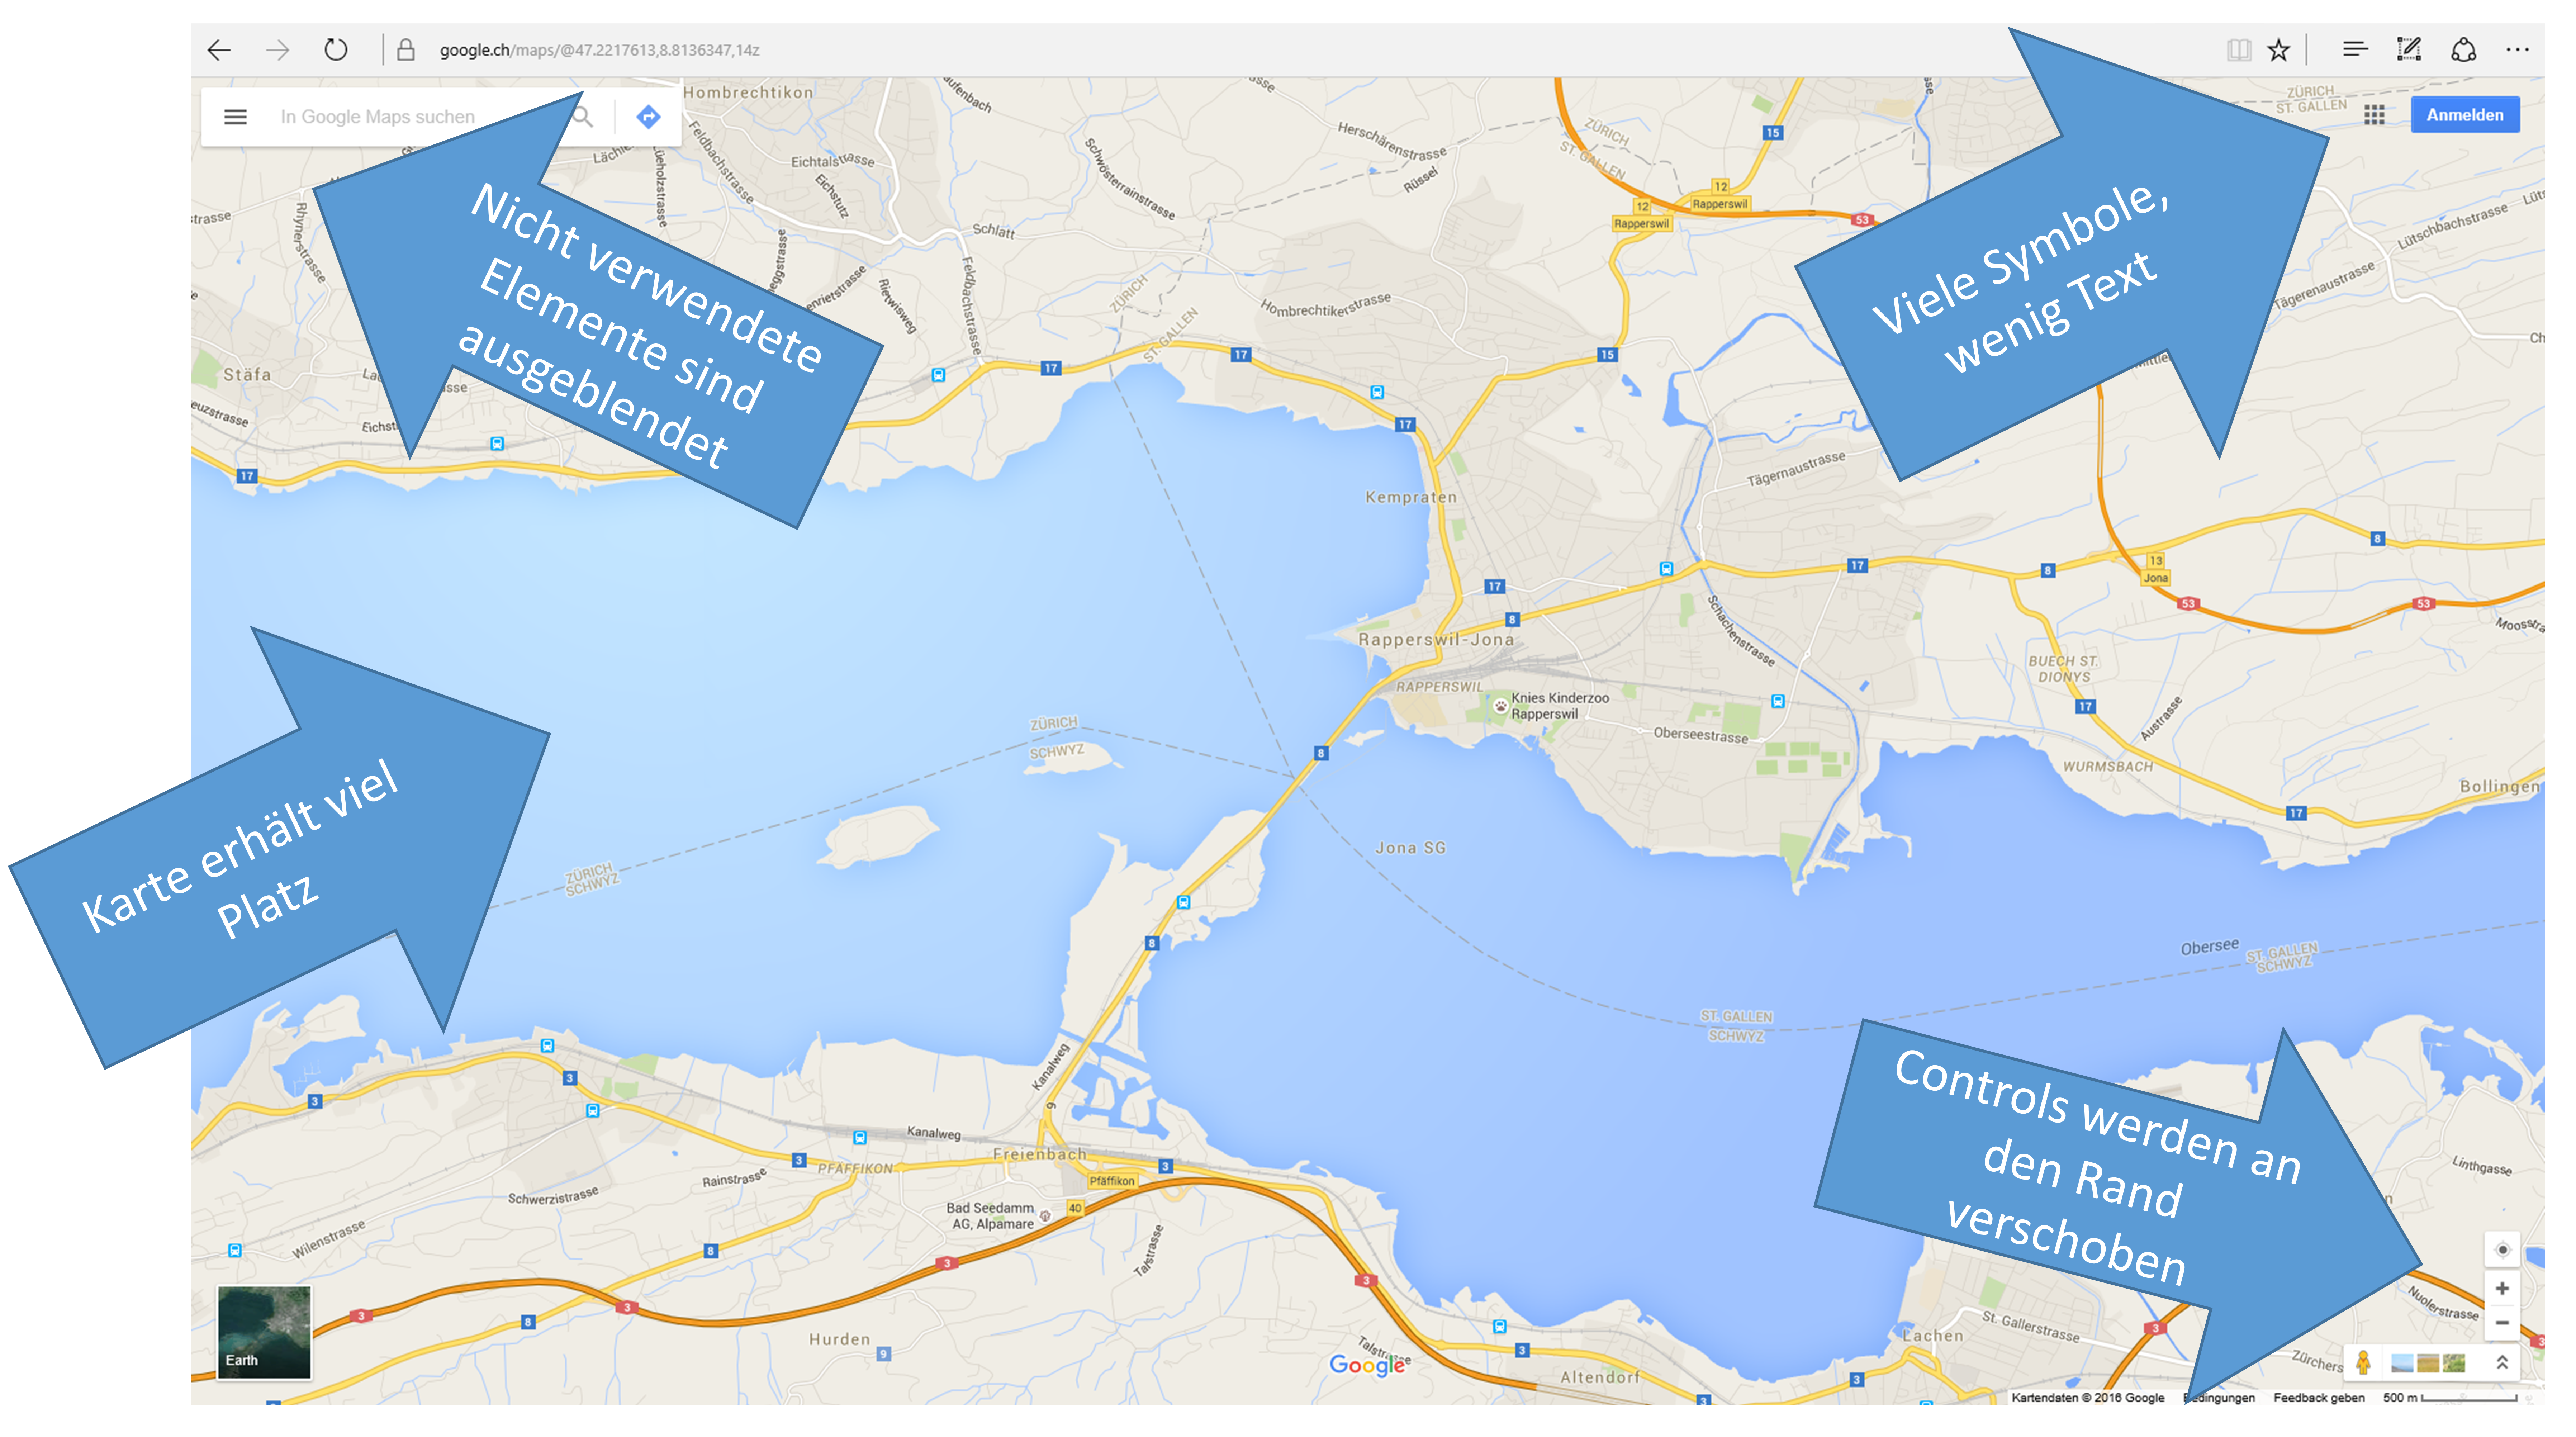
\includegraphics[height=7cm]{images/AnalyseGoogle.png}
\caption{Analyse Google Maps}
\label{fig:googlemaps}
\end{figure}
\noindent
Die Abbildung \ref{fig:googlemaps} \nameref{fig:googlemaps} zeigt die Auswertung der Analyse von Google Maps. Die Karte selbst, erhält sehr viel Platz und alle Bedienelemente (Controls) werden am Randbereich der Karte angeordnet. Dadurch ist sichergestellt, dass sich der Benutzer auf eine Kernaufgabe konzentriert und sich nicht ablenken lässt. Bei schlechteren Beispielen, auf denen die Karte nur wenig Platz erhält, fühlt sich der Benutzer sehr schnell eingegrenzt und muss deutlich mehr Aufwand ins Zoomen und seitlich Bewegen investieren. Dies kann einen Benutzer stören und ihn vom schnellen Erledigen der Aufgabe abhalten. Das User Interface passt sich laufend an die Nutzung des Benutzers an. Hat der Benutzer also einen Ort gefunden und möchten eine Route berechnen, wird ihm neu ein Menü eingeblendet, das ihm dies ermöglicht. Dadurch wird zwar der Karte Platz genommen, jedoch liegt nun das Hauptaugenmerk auf dem Planen der Route. Zusätzlich zum Einsparen von Platz werden bei den Bedienelementen meist kein Text sondern Symbole eingesetzt.
\subsubsection*{Ergebnisse Analyse}
Folgende Punkte, fliessen in das Design des Verkehrsmodell-Fallstudien-Editors mit ein:
\begin{itemize}
\itemsep0em
\item Der Karte viel Platz einräumen.
\item Menüs, welche nicht dem aktuellen Use Case entsprechen, ausblenden.
\item Viele Symbole, wenig Text.
\end{itemize}
\newpage
\subsubsection{ID Editor}
Der ID Editor von OpenStreetMap ist der bekannteste Editor für OpenStreetMap. Er bietet die Möglichkeit Daten von OpenStreetMap direkt auf einer Karte zu bearbeiten. Die Änderungen werden dann als Changeset an OpenStreetMap übertragen und freigeschaltet. Die Funktionalität des Verkehrsmodell-Fallstudien-Editors ähnelt sehr stark den Funktionen des ID Editors. Aufgrund dessen wurde das User Interface des ID Editors ebenfalls analysiert.
\begin{figure}[H]
\centering
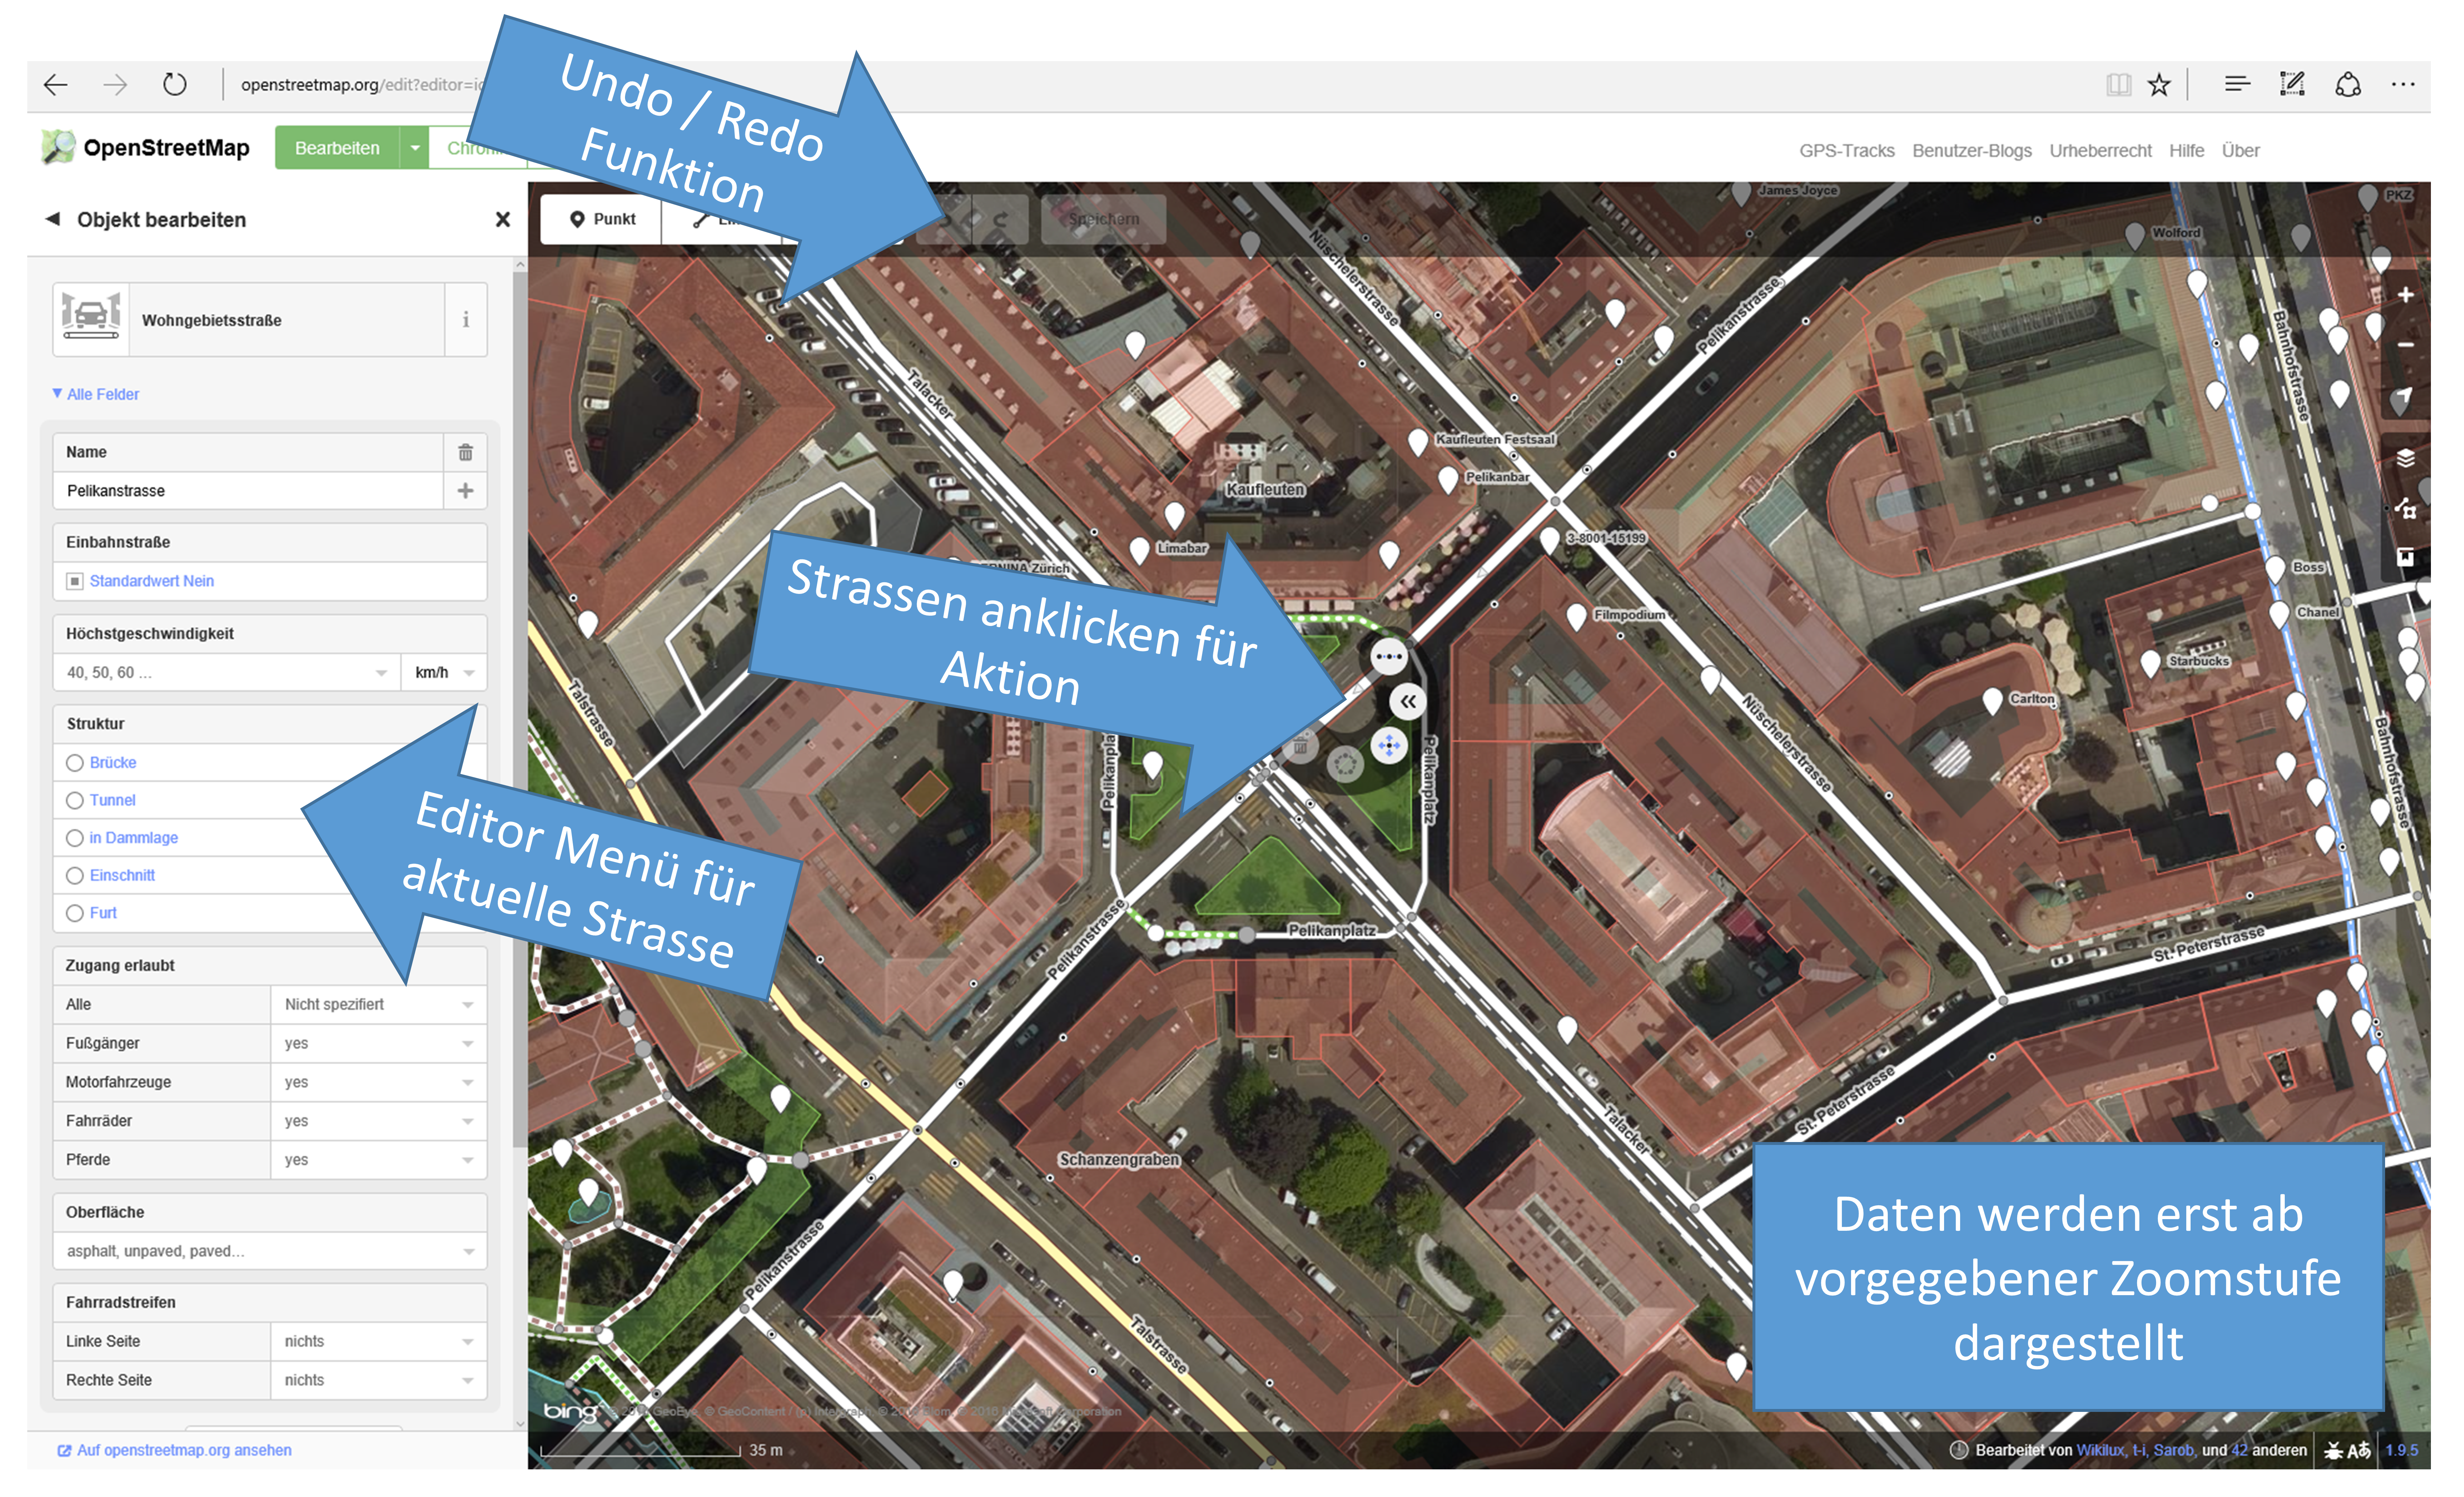
\includegraphics[height=7cm]{images/AnalyseIDEditor.png}
\caption{Analyse ID Editor}
\label{fig:ideditor}
\end{figure}
\noindent
Die Abbildung \ref{fig:ideditor} \nameref{fig:ideditor} zeigt die Auswertung der Analyse des ID Editor. Eine Kerneigenschaft des User Interfaces ist es, dass die Daten erst ab einer gewissen Zoomstufe angezeigt werden. Dies hauptsächlich, weil der ID Editor eine deutlich grössere Datenmenge verarbeiten muss. Diese Eigenschaft ermöglicht es dem ID Editor, die Datenmenge, die zur selben Zeit dargestellt werden muss, auf ein Minimum zu reduzieren. Das Bearbeitungsmenü (Editor Menü) ist so aufgebaut, dass es nach dem Auswählen eines Elements die dazugehörigen Daten des Elements zur Bearbeitung anzeigt. Die Tatsache, dass die Karte dabei immer ersichtlich bleibt, ermöglicht eine leichte und schnelle Bedienung für den Benutzer. Eine weitere wichtige Funktion des ID Editors ist die Undo- / Redo-Funktion. Änderungen an Elementen können einfach wieder rückgängig gemacht werden oder dann wiederhergestellt werden.
\subsubsection*{Ergebnisse Analyse}
Folgende Punkte, fliessen in das Design des Verkehrsmodell-Fallstudien-Editors mit ein:
\begin{itemize}
\itemsep0em
\item Karte bleibt stehen, während Bearbeitung von Strassenattributen.
\item Bearbeitung der Strassen, durch Auswahl.
\item Undo- / Redo-Funktion.
\end{itemize}
\newpage
\subsubsection{Detail Konzept}\label{sec:detailuiconcept}
Aus den Erkenntnissen der Analyse von Google Maps und dem ID Editor wurde folgendes Konzept für das User Interface des Verkehrsmodell-Fallstudien-Editors entwickelt.
\begin{figure}[H]
\centering
\includegraphics[height=7cm]{images/KonzeptUI.png}
\caption{Wireframe Editor}
\label{fig:conceptui}
\end{figure}
\noindent
Angelehnt an Google Maps, wir das User Interface eine Karte besitzen, die den gesamten Platz im Browser ausfüllt. Die Bedienelemente, in der linken oberen Ecke, werden als selbsterklärende Symbole dargestellt und sind während der gesamten Benutzung der Applikation ersichtlich. Menüs, die zur Zeit nicht gebraucht werden, sind, wie in Abbildung \ref{fig:conceptui} dargestellt, ausgeblendet. Dies bietet dem Benutzer viel Platz, für das Suchen und Auswählen einer für ihn relevanten Strasse. Durch das Auswählen einer Strasse, wird ein Menü von der rechten Seite her eingeblendet, das das Bearbeiten der Parameter dieser Strasse ermöglicht (sh. Abbildung \ref{fig:concepteditStreet}).
\begin{figure}[H]
\centering
\includegraphics[height=7cm]{images/KonzeptEditStreet.png}
\caption{Wireframe Strassenattribute bearbeiten}
\label{fig:concepteditStreet}
\end{figure}
\newpage
\noindent
Um die Wegführung einer Strasse zu bearbeiten kann der Benutzer in einen Bearbeitungsmodus wechseln. In diesem Modus werden zusätzlich zu den Links auch die Nodes angezeigt, die ansonsten aus Performancegründen nicht geladen werden. Der Benutzer kann eine Strasse auswählen und dessen Führung mit Hilfe eines Menüs ändern.
\begin{figure}[H]
\centering
\includegraphics[height=7cm]{images/KonzeptChangeStreet.PNG}
\caption{Wireframe Strassenführung bearbeiten}
\label{fig:concepteditStreet}
\end{figure}
\noindent
Ein weiteres, naheliegendes Konzept für die Bearbeitung der Strassenführung, wäre ein Drag \& Drop Verfahren. Dieses Konzept wäre für den Benutzer am einfachsten, ist jedoch sehr zeitintensiv in der Implementation. Aus Zeitgründen musste dadurch auf Drag \& Drop verzichtet werden.
\section{Architektur}
\begin{figure}[H]
\centering
\includegraphics[height=10cm]{images/Architektur.png}
\caption{Tier des Verkehrsmodell-Fallstudien-Editor}
\label{tier_architecture}
\end{figure}
Durch die Anforderungen bezüglich Performance und Antwortgeschwindigkeiten musste die Architektur für die Softwarelösung des Verkehrsmodell-Fallstudien-Editor skalierbar aufgebaut werden. Eine Entkopplung der Komponenten erlaubt eine Verteilung und kann daher die Last auf dem einzelnen Server senken. Die Softwarelösung für den Verkehrsmodell-Fallstudien-Editor ist daher als 3-Tier Applikation aufgebaut. Der Frontside-Tier ist ein Webprojekt implementiert mit dem Play Framework. Der Backend-Tier wird als REST Service (Maturity Level 2) mit Dropwizard entwickelt. Der Daten-Tier wird durch eine PostgreSQL Datenbank bereitgestellt. Der Backend-Tier wird durch eine Load Balancer skalierbar und kann daher mehrere Anfragen parallel ausführen.\\
\begin{figure}[H]
\centering
\includegraphics[height=10cm]{images/layers.png}
\caption{Tier- / Layeraufteilung}
\label{fig:tierlayers}
\end{figure}
\noindent
Die Aufteilung der Presentation Logic auf den Client-Tier, sowie den Backend-Tier erlaubt es die Last der Datendarstellung auf die verschiedenen Komponenten zu verteilen. Die Vorbereitung und Aufbereitung der Daten wird vom Backend-Tier vorgenommen. Die Daten werden im für den Client lesbaren Format übertragen. Das Rendering der Daten übernimmt dann der Client, was dazu führt, dass der Server bei diesen Aufgaben entlastet wird.
\newpage
\section{SimMapEditor}
\begin{figure}[H]
\centering
\includegraphics[height=2cm]{images/presentationlayer.png}
\caption{SimMapEditor}
\label{fig:presentationlayer}
\end{figure}
\noindent
Der SimMap-Editor ist die Frontend-Komponente der Architektur und basiert auf dem Play Framework. Der Client Tier ist eine in Javascript entwickelte Software, welche auf den Backend-Tier zugreift, um die Daten auf der Karte darzustellen. Dabei übernimmt der Client-Tier das Rendering der Daten.
Der SimMapEditor ist die Frontend-Komponente der Achitektur. Der Client Tier wird in Javascript entwickelt und wird als Play Framework Projekt erstellt. Der Client Tier besitzt jedoch keine eigene Business Logic. Diese wird auf den Backend Tier ausgelagert und ist daher nicht im Play Framework implementiert. Der Client Tier ist dafür zuständig das UI Konzept (sh. \ref{sec:uiconcept} \nameref{sec:uiconcept}) zu implementieren und die Daten für die Karte vom Backend Tier anzufordern. Dazu muss der Client Tier das Tilesystem (sh. \ref{ch:datentiles} \nameref{ch:datentiles} ) implementieren und die Daten nach Tiles vom Backend Tier abfragen.
\section{SimMapService}
\begin{figure}[H]
\centering
\includegraphics[height=5.5cm]{images/BusinessLogicLayer.png}
\caption{SimMapService}
\label{fig:businesslogiclayer}
\end{figure}
\noindent
Der SimMapService implementiert den Backend Tier der Softwarelösung in einer 3 Layer Architektur. Er wird als REST Service (Maturity Level 2 \cite{RESTMaturity} ) entwickelt. Um dem Maturity Level 2 zu entsprechen, werden die Anfragen und Antworten des Services mit HTTP Standard Methoden und Codes ausgestattet. Mit den Codes wird dem Client angezeigt, welchen Status die Antwort hat. Z.B. Wird bei einer erfolgreichen Abfrage, welche keine Daten zurückgibt, der Code 201 No Content zurückgesendet. Dies zeigt dem Client, dass er keine Daten erwarten soll, sondern vorgesehen ist das der Body der Antwort leer ist. Für den Aufbau der Antworten mit den korrekten Codes und Umwandlung der Objekte in JSON ist der Presentation Logic Layer des SimMapService zuständig.\\
Der Application Logic Layer des SimMapService ist dafür zuständig die Daten zusammenzufügen und die Preprocessings, welche im Kapitel \ref{sec:concept_preprocessing} \nameref{sec:concept_preprocessing} beschrieben sind, durchzuführen. Er lädt Daten aus dem Resource Layer je nach Zoomlevel und Koordinaten, bereitet dann die Daten auf und übergibt sie dem Presentation Logic Layer.\\
Der Resource Logic Layer bietet dem Application Logic Layer alle Methoden, welche für den Datenzugriff genutzt werden müssen. Seine Aufgabe ist die Erstellung und Durchführung der Abfragen auf die Datenbank.
\section{Datenbank}
\begin{figure}[H]
\centering
\includegraphics[height=2cm]{images/Database.png}
\caption{Datenbank}
\label{fig:database}
\end{figure}
\noindent
Wegen der grossen Datenmenge welche mit der Softwarelösung des Verkehrsmodell-Fallstudien-Editor verwaltet werden soll, ist die Datenbank ein essenzieller Teil der Architektur. Das Datenmodell wurde darauf ausgelegt die Datenmenge der Stammdaten, von den Daten der Changesets (sh. \ref{sec:changeset} \nameref{sec:changeset}) zu trennen. Dadurch wird die Zugriffszeit auf die Stammdaten nicht durch die Datenmenge der User beeinflusst, sondern bleibt unabhängig.
\begin{figure}[H]
\centering
\includegraphics[height=10cm]{images/SimmapDatabase.jpg}
\caption{ERP der Datenbank}
\label{fig:databasescheme}
\end{figure}
\noindent
Im Datenbankschema (Abbildung \ref{fig:databasescheme}) ist ersichtlich, dass die zentrale Komponente der Daten das Network ist. Das Network wird aus einem XML generiert, welches über den Service importiert wird. Ein Network enthält Links und Nodes welche zusammen die Strassen des Strassennetzwerks bilden. In der Tabelle Network\textunderscore Options werden generelle Eigenschaften innerhalb des XMLs gespeichert.\\
Die Tabellen Node\textunderscore Change, Link\textunderscore Change sowie Changeset bilden eine parallele Datenstruktur zu Node und Link. In diesen 3 Tabellen werden die Changesets abgespeichert. Dabei wird nur die Differenz zum Originaldatensatz eingetragen.\\
Das Datenmodell enthält bewusst einige Redundanzen. Diese wurde aus Performancegründen eingeführt. Im Kapitel \ref{ch:redundance} \nameref{ch:redundance} werden die Gründe dazu, genauer erläutert.
